

\section{Introduction}\label{sec:introduction}
%\addcontentsline{toc}{section}{Introduction}
\textbf{\uppercase{The International Data Spaces (IDS) is a virtual data space leveraging existing standards and technologies, as well as governance models well-accepted in the data economy, to facilitate secure and standardized data exchange and data linkage in a trusted business ecosystem. It thereby provides a basis for creating smart-service scenarios and facilitating innovative cross-company business processes, while at the same time guaranteeing data sovereignty for data owners.}}


\subsection{Goals of the International Data Spaces}\label{subsec:Goals_of_IDS}
%\addcontentsline{toc}{subsection}{Goals of the International Data Spaces}
Data sovereignty is a central aspect of the International Data Spaces. It can be defined as a natural person’s or corporate entity’s capability of being entirely self-determined with regard to its data. The International Data Spaces initiative proposes a Reference Architecture Model for this particular capability and related aspects, including requirements for secure and trusted data exchange in business ecosystems.


Overall, there are three types of activities in which the work of the International Data Spaces initiative can be grouped: 1) research activities, 2) standardization activities, and 3) activities for the development of products and solutions for the market (see Figure \ref{fig:_Three_types_of_activities_of_the_International_Data_Spaces}): 

\begin{enumerate}
	\item Fraunhofer runs the Strategic Initiative Data Spaces as a large internal research program aiming at the design and continuous development of the core principles of the IDS Reference Architecture Model (IDS-RAM). An increasing number of further research projects conducted by various partners complement these activities.  


	\item  The International Data Spaces Association (IDSA), a non-profit organization, aims at promoting the IDS-RAM in order to establish an international standard. To achieve this goal, the Association pools the requirements from various industries and provides use cases to test the results gained from the model’s implementation. The standard is intended to materialize in the IDS-RAM itself, but also in defined methods for secure data exchange and data sharing facilitated by the IDS Connector, the central technical component of the International Data Spaces. To ensure the international ambition of the initiative, Regional Hubs have been established in different countries. In addition, the activities of the IDSA aim at supporting the adoption of IDS concepts and technologies in the market. 

	\item Actors in the market can make use of the International Data Spaces standard for providing software services and technology to the market. These products and solutions form the operational IDS ecosystem. As each offering must comply with the International Data Spaces standard, it must undergo a certification process. Therefore, the market requires offerings from evaluation and certification facilities.
\end{enumerate}



%%%%%%%%%%%%%%%%%%%% Figure/Image No: 3 starts here %%%%%%%%%%%%%%%%%%%%

\begin{figure}[H]
	\begin{Center}
		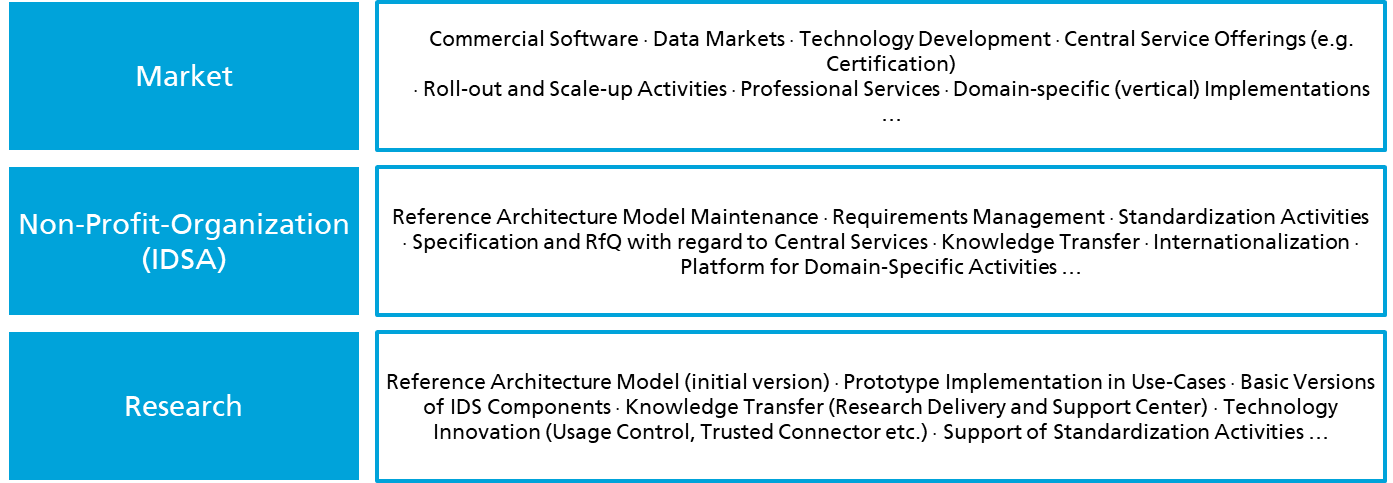
\includegraphics[width=6.35in,height=2.2in]{./media/image10.png}
		\caption{ Three types of activities of the International Data Spaces}
		\label{fig:_Three_types_of_activities_of_the_International_Data_Spaces}
	\end{Center}
\end{figure}


%%%%%%%%%%%%%%%%%%%% Figure/Image No: 3 Ends here %%%%%%%%%%%%%%%%%%%%


The International Data Spaces aims at meeting the following strategic requirements:


\begin{itemize}
	\item \textbf{Trust}: Trust is the basis of the International Data Spaces. Each participant is evaluated and certified before being granted access to the trusted business ecosystem.
	%ToDo: Update this section to general reference to research projects.

	\item \textbf{Security and data sovereignty}: All components of the International Data Spaces rely on state-of-the-art security measures. Apart from architectural specifications, security is mainly ensured by the evaluation and certification of each technical component used in the International Data Spaces. In line with the central aspect of ensuring data sovereignty, a data owner in the International Data Spaces attaches usage restriction information to their data before it is transferred to a data consumer. To use the data, the data consumer must fully accept the data owner’s usage policy.

	\item \textbf{Ecosystem of data}: The architecture of the International Data Spaces does not require central data storage capabilities. Instead, it pursues the idea of decentralization of data storage, which means that data physically remains with the respective data owner until it is transferred to a trusted party. This approach requires a comprehensive description of each data source and the value and usability of data for other companies, combined with the ability to integrate domain-specific data vocabularies. In addition, brokers in the ecosystem provide services for real-time data search.

	\item \textbf{Standardized interoperability}: The International Data Spaces Connector, being a central component of the architecture, is implemented in different variants and can be acquired from different vendors. Nevertheless, each Connector is able to communicate with any other Connector (or other technical component) in the ecosystem of the International Data Space.

	\item \textbf{Value adding apps:} The International Data Spaces allows to inject apps into the IDS Connectors in order to provide services on top of data exchange processes. This includes services for data processing, data format alignment, and data exchange protocols, for example. Furthermore, data analytics services can be provided by remote execution of algorithms.

	\item \textbf{Data markets}: The International Data Space enables the creation of novel, data-driven services that make use of data apps. It also fosters new business models for these services by providing clearing mechanisms and billing functions, and by creating domain-specific broker solutions and marketplaces. In addition, the International Data Spaces provides templates and other methodological support for participants to use when specifying usage restriction information and requesting legal information. 

\end{itemize}

%ToDo: dereference from reseearch project
\textbf{Being the central deliverable of the research project, the Reference Architecture Model of the International Data Spaces (IDS-RAM) constitutes the basis for a variety of software implementations, and thus for a variety of commercial software and service offerings.}


\textbf{All research and development activities, as well as all activities with regard to standardization, are driven by the following guidelines:}

\begin{itemize}

	\item \textbf{Open development process}: The International Data Spaces Association is a non-profit organization institutionalized under the German law of associations. Every organization is invited to participate, as long as it adheres to the common principles of work.

	\item \textbf{Re-use of existing technologies}: Inter-organizational information systems, data interoperability, and information security are well-established fields of research and development, with plenty of technologies available in the market. The work of the International Data Spaces initiative is guided by the idea not to $``$reinvent the wheel$"$ , but to use existing technologies (e.g., from the open-source domain) and standards (e.g., semantic standards of the W3C) to the extent possible.

	\item \textbf{Contribution to standardization}: Aiming at establishing an international standard itself, the International Data Spaces initiative supports the idea of standardized architecture stacks.

\end{itemize}


\subsection{Purpose and Structure of the Reference Architecture Model}\label{subsec:purpose_of_ram}
%\addcontentsline{toc}{subsection}{Purpose and Structure of the Reference Architecture Model}
Focusing on the generalization of concepts, functionality, and overall processes involved in the creation of a secure $``$network of trusted data$"$ , the IDS-RAM resides at a higher abstraction level than common architecture models of concrete software solutions do. The document provides an overview supplemented by dedicated architecture specifications defining the individual components of the International Data Spaces (Connector, Broker, App Store, etc.) in detail.

In compliance with common system architecture models and standards (e.g., ISO 42010, 4+1 view model), the Reference Architecture Model uses a five-layer structure expressing various stakeholders’ concerns and viewpoints at different levels of granularity.

%ToDo: link sections here
The general structure of the Reference Architecture Model is illustrated in Figure \ref{fig:_General_structure_of_Reference_Architecture_Model}. The model is made up of five layers: The \textit{Business Layer} specifies and categorizes the different roles which the participants of the International Data Spaces can assume, and it specifies the main activities and interactions connected with each of these roles. The \textit{Functional Layer} defines the functional requirements of the International Data Spaces, plus the concrete features to be derived from these. The \textit{Process Layer} specifies the interactions taking place between the different components of the International Data Spaces; using the BPMN notation, it provides a dynamic view of the Reference Architecture Model. The \textit{Information Layer} defines a conceptual model which makes use of linked-data principles for describing both the static and the dynamic aspects of the International Data Space’s constituents. The \textit{System Layer} is concerned with the decomposition of the logical software components, considering aspects such as integration, configuration, deployment, and extensibility of these components.

In addition, the Reference Architecture Model comprises three perspectives that need to be implemented across all five layers: \textit{Security}, \textit{Certification}, and \textit{Governance}. 



%%%%%%%%%%%%%%%%%%%% Figure/Image No: 4 starts here %%%%%%%%%%%%%%%%%%%%

\begin{figure}[H]
	\begin{Center}
		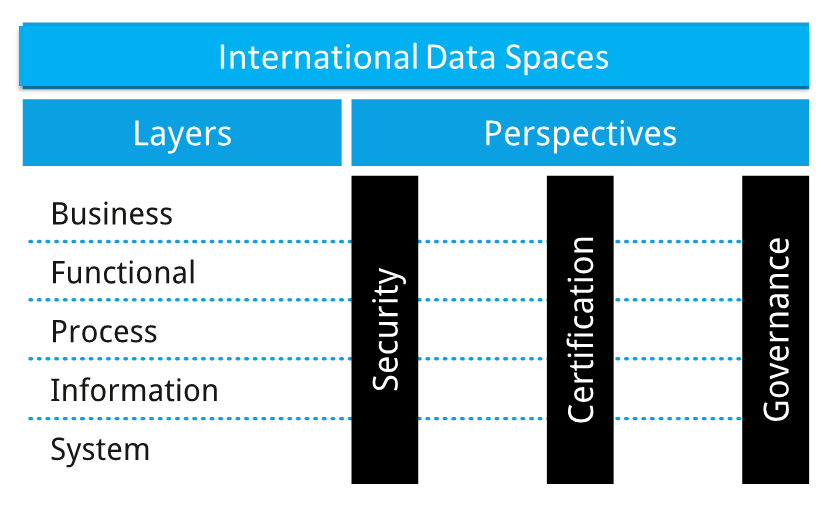
\includegraphics[width=4.12in,height=2.58in]{./media/image11.png}
		\caption{ General structure of Reference Architecture Model}
		\label{fig:_General_structure_of_Reference_Architecture_Model}
	\end{Center}
\end{figure}


%%%%%%%%%%%%%%%%%%%% Figure/Image No: 4 Ends here %%%%%%%%%%%%%%%%%%%%
